% !TEX root = ../main.tex
\clearpage
\phantomsection
\section*{4 \textbf{Theoretical Framework}}
\label{sec:theoretical-framework}
\addcontentsline{toc}{section}{4 Theoretical Framework}

This study is grounded in hyperlink-citation theory, predictive validity, and computational complexity theory to compare EndorseRank against Adaptive Weighted PageRank (AWP) across three core constructs: Reputation Structure, Risk Predictive Validity, and Computational Efficiency. Each construct links directly to the parameter definitions introduced earlier in the research objectives and expected-results framework and supports testable hypotheses.


\phantomsection
\subsection*{4.1 Constructs and Variable Mapping}
\label{sec:constructs-and-variable-mapping}
\addcontentsline{toc}{subsection}{4.1 Constructs and Variable Mapping}

\begin{longtable}{>{\raggedright\arraybackslash}p{0.25\linewidth}>{\raggedright\arraybackslash}p{0.36\linewidth}>{\raggedright\arraybackslash}p{0.29\linewidth}}
\caption{Evaluation Constructs and Associated Variables}\\
\toprule
\textbf{Construct} & \textbf{Associated variables} & \textbf{Operational measures} \\
\midrule
Reputation Structure & EndorseRank score, AWP score, rank ordering, rank divergence & Spearman's rho, Kendall's tau, top-k overlap \\
\addlinespace
Risk Predictive Validity & Default/liquidation label and score-based prediction features & AUC, precision, recall, F1-score, calibration \\
\addlinespace
Computational Efficiency & Graph build time, PageRank convergence time, memory usage, iteration count & Runtime, peak memory, iterations to tolerance \\
\addlinespace
\bottomrule
\end{longtable}

\phantomsection
\subsection*{4.2 Conceptual Model}
\label{sec:conceptual-model}
\addcontentsline{toc}{subsection}{4.2 Conceptual Model}

\begin{center}
% !TEX root = ../main.tex
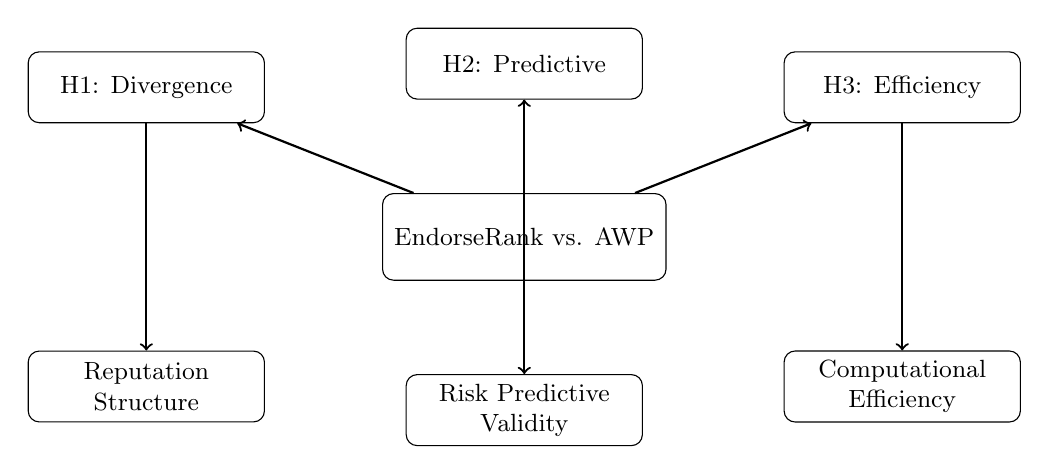
\begin{tikzpicture}[
  font=\small,
  box/.style={draw, rounded corners, align=center, minimum width=3.6cm, minimum height=1.1cm},
  smallbox/.style={draw, rounded corners, align=center, minimum width=3.0cm, minimum height=0.9cm},
  arrow/.style={->, thick}
]
\node[box] (center) at (0,0) {EndorseRank vs. AWP};
\node[smallbox] (h1) at (-4.8,1.9) {H1: Divergence};
\node[smallbox] (rep) at (-4.8,-1.9) {Reputation\\Structure};
\node[smallbox] (h2) at (0,2.2) {H2: Predictive};
\node[smallbox] (risk) at (0,-2.2) {Risk Predictive\\Validity};
\node[smallbox] (h3) at (4.8,1.9) {H3: Efficiency};
\node[smallbox] (eff) at (4.8,-1.9) {Computational\\Efficiency};
\draw[arrow] (center) -- (h1);
\draw[arrow] (center) -- (h2);
\draw[arrow] (center) -- (h3);
\draw[arrow] (h1) -- (rep);
\draw[arrow] (h2) -- (risk);
\draw[arrow] (h3) -- (eff);
\end{tikzpicture}

\end{center}


\begin{center}Figure 1: EndorseRank vs. AWP: hypotheses and evaluation constructs\end{center}

\textbf{H1 (Divergence): }EndorseRank and AWP will yield significantly different wallet orderings, demonstrating that an approve/permit--based endorsement graph creates a distinct reputation structure.


\textbf{H2 (Predictive Validity): }EndorseRank's scores will correlate more strongly with actual default events than AWP's scores, indicating superior predictive power.


\textbf{H3 (Computational Efficiency): }EndorseRank will require less runtime, memory, and fewer iterations to converge than AWP, demonstrating practical scalability advantages.


\phantomsection
\subsection*{4.3 Theoretical Justification}
\label{sec:theoretical-justification}
\addcontentsline{toc}{subsection}{4.3 Theoretical Justification}

\textbf{Hyperlink--Citation Semantics: }The original PageRank algorithm (Page et al., 1998) evaluates a webpage's importance by the structure of inbound hyperlinks, treating each link like a citation in an academic paper: pages that are linked to by many important pages receive higher rank. ERC- 20 approve/permit edges can be interpreted similarly, where an approval from wallet A to wallet B functions as a trust citation, justifying the use of PageRank on an approval graph.


\textbf{Predictive Validity Framework: }In credit scoring and psychometrics, predictive validity assesses how well a metric forecasts real-world outcomes.


By treating EndorseRank and AWP scores as assessment scales, we employ standard metrics (AUC, Precision, Recall, F1-score) to compare their ability to predict defaults.


\textbf{Computational Complexity Theory: }PageRank's time complexity per iteration is O(---E---). Approve/permit graphs are sparser than transfer- based graphs (fewer edges ---E---), leading to lower per-iteration cost, faster convergence, and reduced memory usage.


\phantomsection
\subsection*{4.4 Implications for Research Design}
\label{sec:implications-for-research-design}
\addcontentsline{toc}{subsection}{4.4 Implications for Research Design}

\textbf{Measurement: }Compute EndorseRank and AWP scores for a matched sample of Aave wallets, record default outcomes over a defined period, and profile each algorithm's runtime, memory usage, and iterations to convergence.


\proposalSubheading{Analysis:}

\textbf{H1 }via rank correlation (Spearman's \emph{\(\rho\)}, Kendall's \emph{\(\tau\)})


\textbf{H2 }via predictive metrics (AUC, Precision, Recall, F1-score)


\textbf{H3 }via paired benchmarks of runtime, peak memory, and iteration counts


\textbf{Contribution: }By anchoring our hypotheses in established theories, this framework ensures that empirical results will offer both scholarly rigor and practical relevance, demonstrating EndorseRank's advantages in producing a semantically meaningful, predictive, and efficient on-chain reputation metric.
